\chapter[IMPLEMENTACION]{IMPLEMENTACIÓN}
En los capitulos anteriores pesentamos impletentaciones de alto nivel de la arquitectura de un sistema un 
conceptual de un sistema de chatbot, asi como tambien arquitecturas recomendadas por la documentación de Rasa. En el presente capitulo presentaremos los componenetes elegidos y sus funciones en el sistema.
  
\section{Docker}

Para construir los servicios se usaron microcontenedores Docker, por lo que intruduciremos brevemente los conceptos de esta tegnologia. 

\subsection{Contenedor}

Los contenedores son la unidad mas pequeña de un servicio, es una entidad que se utiliza para aislar cada componente del sistema base. Cada contenedor puede aislarse mediante funciones del sistema operativo llamadas cgroups y cnames logrando asi aplicaciones en entornos aislados (sandboxed en Ingles). \cite{Docker}   

\begin{figure}[ht]
    \centering
    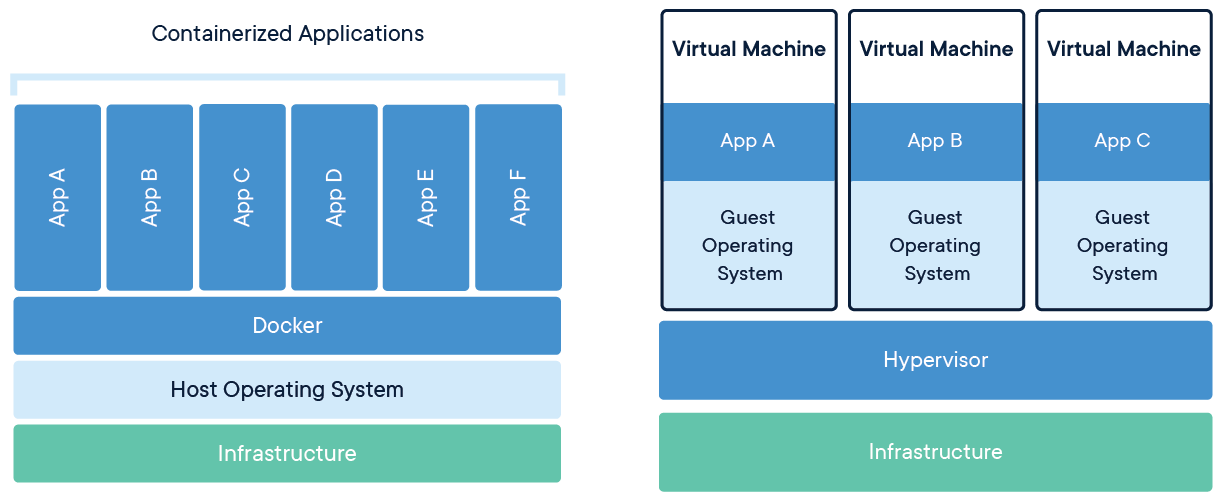
\includegraphics[width=\textwidth]{imagenes/cap4/docker-container.png}
    \caption{Contenedores}
    \label{fig:container_diagram}
\end{figure}


\subsection{Imagen de contenedor}

Una imagen de contenedor es el sistema de arhivos aislados de todos los archivos necesarios para ejecutar la aplicacion asi como dependecias, configuraciones, executables, etc. Asi como tambien variables de entorno y datos necesarios para ejecutar la aplicación. \cite{Docker}  

\subsection{Redes}

Entre las ventajas de desplegar una aplicación por medio de contenedores docker es que se pueden comunicar entre ellos y tambien con sevicios externos al entorno de Docker. Por defecto se pueden crear varios tipos de configuraciones de red, pero por lo general se utilizan redes puente entre los contenedores para que estos puedan comunicarse mutuamente entre ellos y solo exponienco los puertos necesarios para interacuar con el sistema en cuestion y esta es la opción utilizada en nuestra implementaón. \cite{Docker}  

\subsection{Volumenes}
Puesto que un contenedor no tiene un estado percistente sobre los datos que genera se introducen los volumenes son la forma recomedada de agregar presistencia de datos a un contendedor de Docker. 
\cite{Docker} 

\begin{figure}[ht]
    \centering
    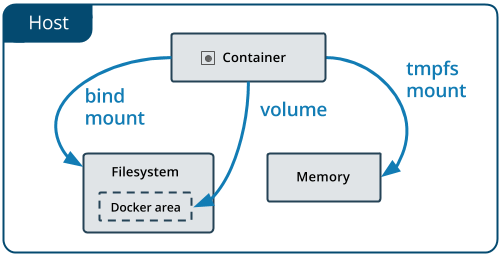
\includegraphics[width=\textwidth]{imagenes/cap4/docker-volume.png}
    \caption{Volumen}
    \label{fig:volume_diagram}
\end{figure}

\subsection{Construción}
Las imagenes de docker se consytruyen apartir de instrucciones escritas en un achivo denominadado Dockerfile, 
generalmente de parte de una imagen base de la cual se le adicciona lo necesario para ejecutar la aplicación.
\cite{Docker}


\subsection{Repositorios}
Un respotorio de imagenes Docker(Docker Registry) es un servidor que almacena y distribuye imagenes versionadas deneradas apartir de un Dockerfile. Estos repositorios pueden ser publicos como DockerHub que es el oficcial de la comunidad de Docker como asi tambien privado para un equipo de desarrollo en una institucion.
\cite{Docker}

\section{Componentes}

Cada componente del sistema se configuro en un contenedor de Docker con la exepcion del servidor NGINX que si estaba instalado sobre el sistema operativo del servidor. 
\begin{figure}[ht]
    \centering
    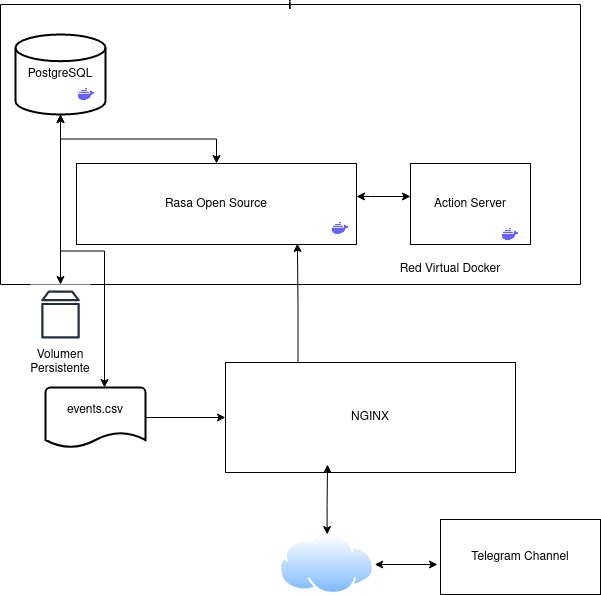
\includegraphics[width=\textwidth]{imagenes/cap4/server.png}
    \caption{Componentes del sistema}
    \label{fig:server_diagram}
\end{figure}


\subsection{Rasa Open Source}

El contendedor de Rasa Open Source ejecuta una imagen oficial proveida por Rasa disponible en los repositorios de DockerHub\cite{DockerHub}, pero con el modelo entrenado y las configureaciones particulares al proyecto. Es el unico conteneor que tiene un puerto externo para servir a los usuario. Tambien hace uso de los servicios de PosgresSQL y de el servicio de acciones(action server). 


\subsection{Servidor de acciones}

Servidor de acciones(acction server) es un servicio interno que ejecuta codigo escrito en python este utiliza una imagen oficial para servicios Python disponible en los repsoitorios de DockerHub\cite{DockerHub}, estos son operaciones especificas para algunas acciones una respuesta no estatica, como por el ejemplo la accion relacionada a el calculo de puntajes en el final deacuardo a los puntajes en los examenes parciales.

 \subsection{PostgresSQL}
  
 PostgresSQL es un motor de base de datos del tipo relacional\cite{postgresql} el cual se configuro apartir de una imagen official de PostgresSQL disponible en los repositorios de DockerHub\cite{DockerHub}. Aparte de sus funciones de base de datos de sistema tambien ejecutra un trabajo periodico(cada una hora) para realizar una copia acualizada de los contenidos de la tabla Eventos a un archivo separado por comas(csv) que se utiliza para realimentar las conversaciones y generar mas datos para mejorar el modelo. 

 \subsection{NGINX}

 NGINX, es una servidor web que tambien puede ser usado como proxy reverso, que implica redirigir el trafico a puertos internos y también para servir archivos que fueron las funciones ulizadas para el proyecto. Asi como tambien puede ser utilizado como balanceador de carga, mail proxy y HTTP cache entre otras funciones \cite{NGINX}
El servidor NGINX redige el trafico a la instancia de Rasa Open Source y si como tambien sirve el archivo de 
la copia mas reciente de la tabla Eventos para agilizar las verificaciones de las respuestas y preguntas recibidas.

\section{Recursos}

Para la puesta en producción de el proyecto, se utilizo una instancia de Droplet alojado en Nueva York del proveedor DigitalOcean con un procesador con un 1vcpu(procesaror virtualizado), 1 GB de ram, 25 GB de alacenamiento y con un costo de entre 4 y 6 dolares americanos al mes dependiendo de el trafico presentado. Por las limitaciones de memoria del servirdor se configuro tambien 4 GB de espacio de intercambio(SWAP) en el espacio de alacenamiento.  

\section{Telegram}

Para habilitar pruebas para el publico general se eligio Telegram, puesto que es bastante sencillo usar su servicio para connectar a implementaciones de chatbot y este no tiene costo por el uso. \cite{botfather}
